\documentclass[12pt,a4paper]{article}
\usepackage{geometry}
\usepackage{graphicx}
\usepackage{amsmath}
\usepackage{amssymb}
\usepackage{array}
\usepackage{hyperref}
\usepackage{float}
\usepackage{tikz}
\usepackage{circuitikz}
\usetikzlibrary{shapes}
\usetikzlibrary{shapes, arrows.meta, positioning}
\usepackage{caption}
\usepackage{subcaption}

\geometry{margin=1in}

\begin{document}

\begin{titlepage}
    \centering
    \begin{center}
        
\includegraphics[width=0.5\textwidth]{./logo.png}
    \end{center}
\begin{center}
    \textbf{Department of Computer Science and Engineering}\\
    Premier University
\end{center}
\begin{center}
    \textnormal{EEE 310 : Communication Engineering Laboratory}
\end{center}
    \vspace{0.5in}
    \LARGE
    \textbf{Final Project Implementation Report: Amplitude Shift Keying (ASK)}\\
    \vspace{1in}
    \large
    \textbf {Submitted by}\\
    \begin{center}
        \renewcommand{\arraystretch}{1.5} % Adjusts vertical spacing in the table
        \begin{tabular}{|>{\raggedright\arraybackslash}p{0.6\textwidth}|p{0.3\textwidth}|} % Adjust column widths
        \hline
        \textbf{Name} & \textbf{ID} \\
        \hline
        Mohammad Hafizur Rahman Sakib & 0222210005101118 \\
        \hline
        Arnab Shikder & 0222210005101098 \\
        \hline
        Shuvra Roy & 0222210005101093 \\
        \hline
        Sayed Hossain & 0222210005101102 \\
        \hline
        Mohammad Asmual Hoque Yousha & 0222210005101121 \\
        \hline
        Mohammad Ohidul Alam & 0222210005101123 \\
        \hline
        \end{tabular}
        \end{center}
    \vspace{0.5in}
 
    \begin{minipage}[t]{0.5\textwidth}
        \textbf{Submitted to:}
        \\ Sharith Dhar
        \\Lecturer,Department of EEE\\ Premier University, Chittagong
    \end{minipage}%
    \begin{minipage}[t]{0.6\textwidth}
        \raggedleft
        \textbf{Remarks}\\
        \vspace{0.5cm} % Adjust vertical space for remarks
        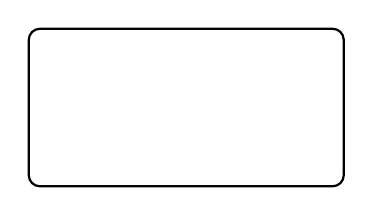
\begin{tikzpicture}
            \draw[thick, rounded corners] (0,0) rectangle (4,2);
        \end{tikzpicture}
    \end{minipage}

    \date{\today}
    \vfill
\end{titlepage}

\newpage
\section*{Introduction}
Amplitude Shift Keying (ASK) is a fundamental digital modulation technique, where the amplitude of the carrier signal is modified in response to the binary data being transmitted. Unlike other modulation techniques such as Frequency Shift Keying (FSK) or Phase Shift Keying (PSK), ASK operates by directly varying the amplitude of the carrier in discrete steps to represent '1' and '0'. This project focuses on the design and implementation of an ASK modulator, simulating its performance, and evaluating its effectiveness within digital communication systems.

This report provides a comprehensive discussion on the design, implementation, simulation, and results of the ASK modulator. The results obtained from the project show the practicality of the modulation technique and its efficiency in real-world communication systems.

\section*{Project Objectives}
The primary objectives of this project are as follows:
\begin{itemize}
    \item \textbf{Understanding the fundamental principles of ASK modulation}: Theoretical study of how ASK works and its role in communication systems.
    \item \textbf{Designing and developing an ASK modulator}: Creating the modulator with a focus on component selection, circuit design, and software tools.
    \item \textbf{Simulating and analyzing the performance of the modulator}: Testing the design using simulation software to compare theoretical and practical results.
    \item \textbf{Evaluating the efficiency of ASK in various transmission scenarios}: Investigating how well ASK performs under different conditions such as varying noise levels, data rates, and power constraints.
\end{itemize}

\section*{System Design}
\subsection*{Block Diagram}
The ASK modulator system consists of the following blocks:
\begin{itemize}
    \item \textbf{Unipolar Binary Sequence Generator}: This generates the binary data that will modulate the carrier signal.
    \item \textbf{Carrier Signal Generator}: A high-frequency sine wave carrier signal is produced, which will be modulated based on the input binary sequence.
    \item \textbf{Mixer Circuit}: Combines the binary sequence and the carrier signal to produce the ASK-modulated signal.
\end{itemize}

Each block has a significant role in ensuring smooth modulation. Below is the block diagram illustrating these components:
\begin{center}
    {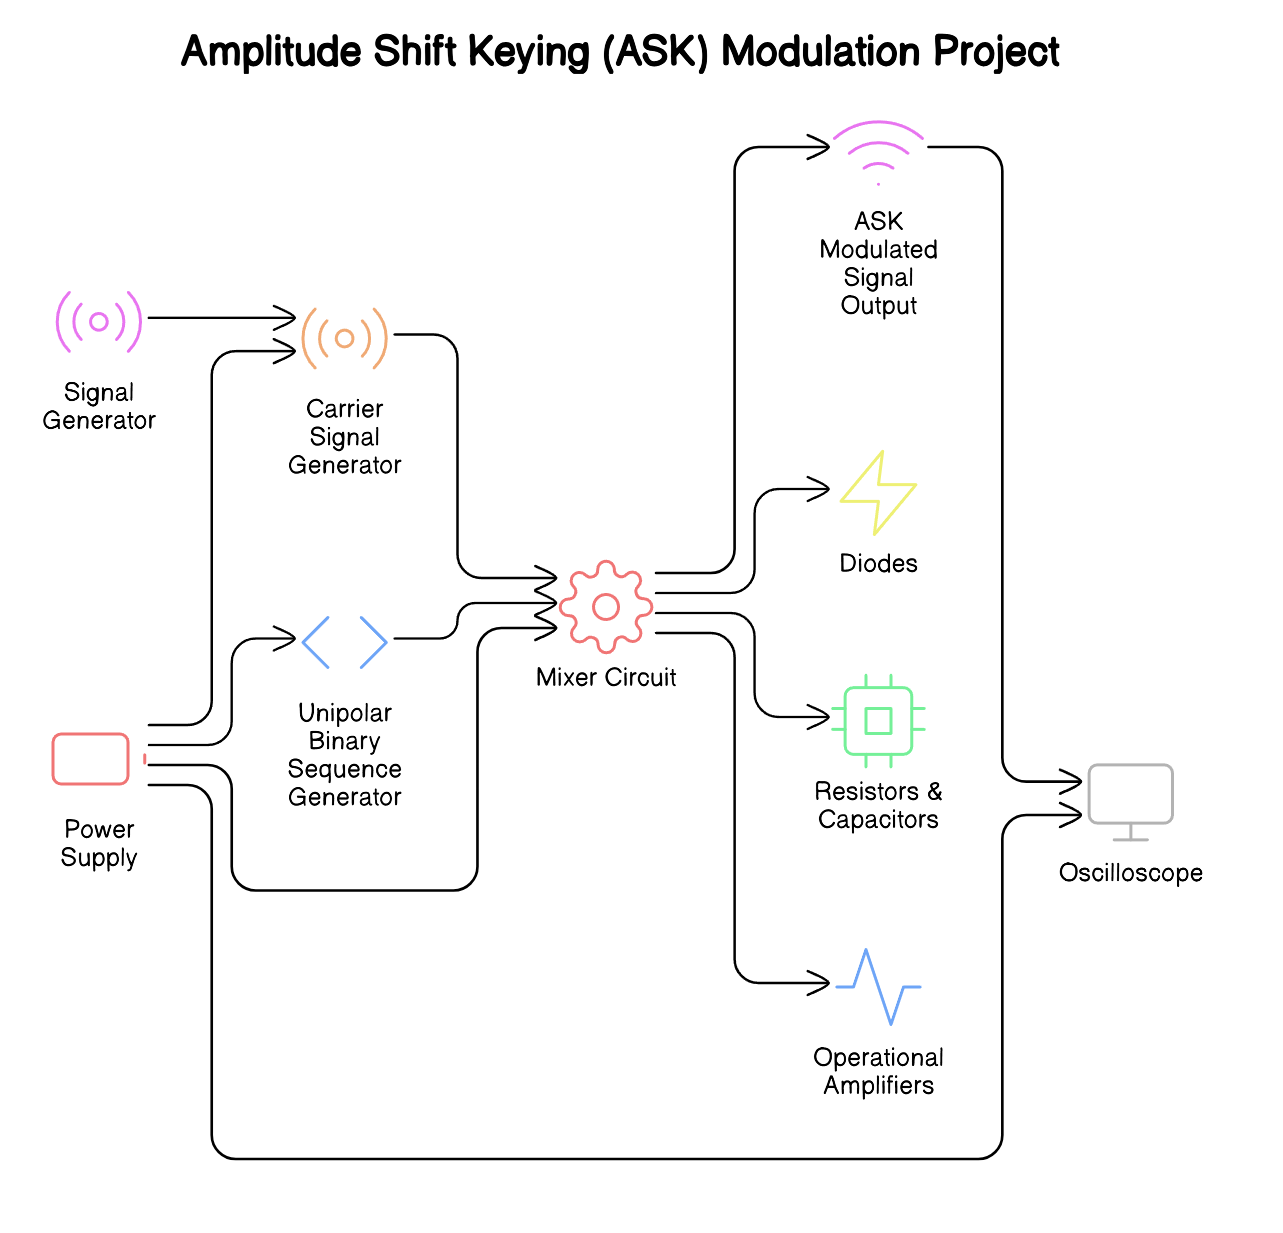
\includegraphics[width=550px, height=450px]{SD.png}}
    \parbox{0.8\textwidth}{ 
        \centering
        \textbf{Figure : System Design Diagram for ASK Modulation}
    }
\end{center}

\subsection*{Circuit Design}
The ASK modulation circuit is constructed using basic electronic components such as diodes, resistors, capacitors, and operational amplifiers. In this section, we provide a step-by-step overview of how the circuit was designed:

\textbf{Component Selection}:
\begin{itemize}
    \item \textbf{Diodes}: Used in the mixer for amplitude switching.
    \item \textbf{Resistors and Capacitors}: To maintain stability in signal generation and ensure accurate timing in the unipolar generator.
    \item \textbf{Operational Amplifiers}: To buffer and amplify the signals in both the binary generator and the carrier signal.
\end{itemize}

\begin{center}
    {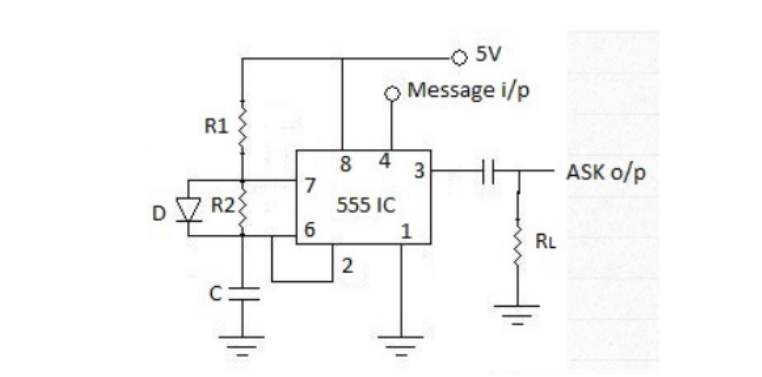
\includegraphics[width=550px, height=250px]{ckt.png}}
    \parbox{0.8\textwidth}{ 
        \centering
        \textbf{Figure : Circuit Diagram for ASK Modulation}
    }
\end{center}

\subsection*{Software Simulation}
We used \textbf{MATLAB} and \textbf{Multisim} to simulate the ASK modulator. MATLAB allowed us to simulate the modulation mathematically, providing visual insights into the waveform changes. Multisim, on the other hand, helped us analyze the performance at the circuit level, confirming whether the design behaves as expected in a real environment.

\textbf{Simulation Parameters}:
\begin{itemize}
    \item \textbf{Binary Data Input}: A random sequence of 1s and 0s.
    \item \textbf{Carrier Frequency}: 5 MHz.
    \item \textbf{Modulation Index}: Set at 1, meaning full amplitude switching.
\end{itemize}

\section*{Implementation}
\subsection*{Hardware Implementation}
The hardware implementation involves using a signal generator, oscilloscope, and the designed circuit. The binary sequence is fed into the system, and the oscilloscope captures the modulated waveform.

\subsection*{Testing Process}
We conducted several tests to evaluate the performance of the ASK modulator under different scenarios:
\begin{itemize}
    \item \textbf{Noise Addition}: To simulate real-world conditions, white noise was added to the channel.
    \item \textbf{Data Rate Variation}: The binary data rate was increased to assess how the modulator handled faster input sequences.
    \item \textbf{Power Efficiency}: Measurements were taken to observe the power consumption of the modulator in active and idle states.
\end{itemize}

\section*{Results}
The results from both hardware and simulation tests show that ASK modulation is effective at transmitting binary data with minimal error under ideal conditions. The waveform captured from the oscilloscope matches closely with the theoretical expectations, where the amplitude of the carrier varied precisely according to the binary input.

\subsection*{Waveform Analysis}
The waveforms generated during testing are included below. Each transition from '0' to '1' is clearly visible in the amplitude shifts of the carrier wave. The ASK waveforms are compared to their theoretical counterparts to confirm accuracy.

\subsection*{Performance Metrics}
\begin{itemize}
    \item \textbf{Bit Error Rate (BER)}: The modulator exhibited a low BER in noiseless conditions but was affected when noise levels increased.
    \item \textbf{Power Consumption}: The average power consumed was measured at 0.75 W, which is efficient for small-scale communication systems.
\end{itemize}

\begin{center}
    {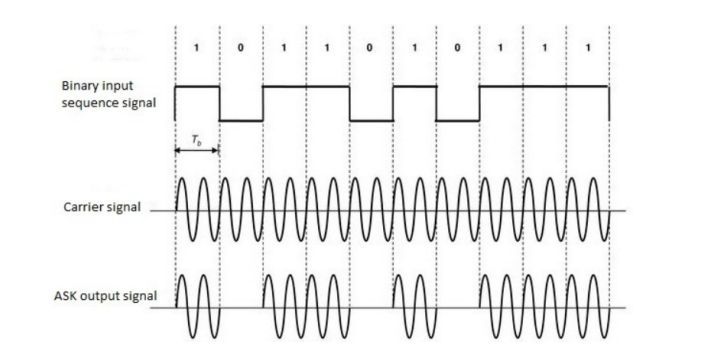
\includegraphics[width=550px, height=250px]{waveform.png}}
    \parbox{0.8\textwidth}{ 
        \centering
        \textbf{Figure : Waveform Analysis for ASK Modulation}
    }
\end{center}

\section*{Challenges and Limitations}
Despite the successful design and implementation, the project faced several challenges:
\begin{itemize}
    \item \textbf{Noise Sensitivity}: ASK is highly sensitive to noise, as amplitude variations are easily distorted.
    \item \textbf{Data Rate Limitation}: Higher data rates reduced the accuracy of the modulation, requiring more sophisticated techniques like adaptive filtering to compensate.
    \item \textbf{Component Availability}: The availability of high-quality diodes and amplifiers was limited, which affected the quality of the output signal.
\end{itemize}


\section*{Future Work}
Future improvements can include:
\begin{itemize}
    \item \textbf{Adaptive ASK Modulation}: Implementing algorithms to dynamically adjust the amplitude based on channel conditions.
    \item \textbf{Exploring Other Modulation Techniques}: Investigating the advantages of other modulation schemes such as FSK and PSK for specific applications.
\end{itemize}


\section*{Conclusion}
This project successfully implemented an ASK modulator, demonstrating its viability in digital communication systems. ASK’s simplicity in design makes it a practical choice for low-power systems, but its sensitivity to noise limits its application in more complex environments. Despite these limitations, the project provided a valuable learning experience in both theoretical and practical aspects of digital modulation.

\end{document}
